\documentclass[letter]{article}

\usepackage{MD_estilo}

\nombre{Matías Duhalde} % Aqui va el nombre del alumno
\lista{-} % Aqui va el numero de lista
\numtarea{2} % Aqui va el número de la tarea

\sigla{IIC2223} % Aqui va la sigla del curso
\curso{Teoría de Autómatas y Lenguajes Formales} % Aqui va el nombre del curso
\semestre{2} % Aqui va el semestre del curso
\ano{2021} % Aqui va el año del curso


\begin{document}
	
\begin{pregunta}{1} % Aqui se coloca el número de la pregunta

\subsection*{ExpReg 1}

\textbf{Todas las palabras que no contienen la subpalabra \textit{abc}.} \\

Para definir esta expresión regular, es mucho más conveniente comenzar desde un autómata. El siguiente DFA define el lenguaje esperado.
\begin{center}
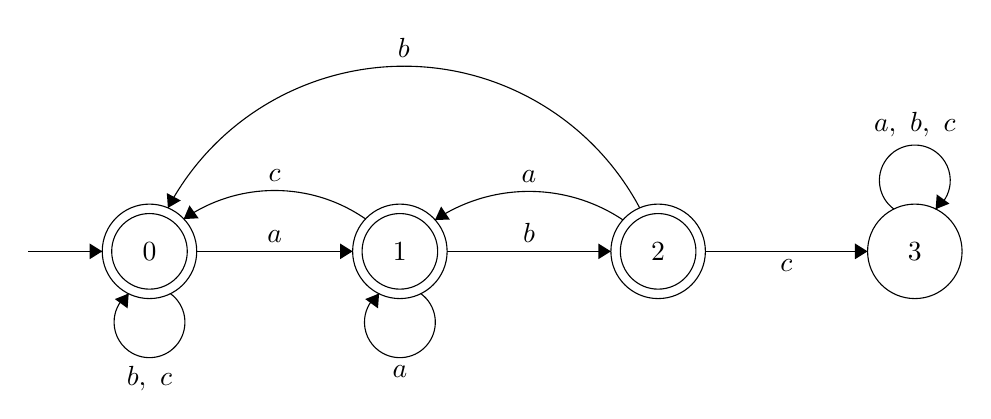
\begin{tikzpicture}[scale=0.2]
\tikzstyle{every node}+=[inner sep=0pt]
\draw [black] (15.1,-27.3) circle (3);
\draw (15.1,-27.3) node {$0$};
\draw [black] (15.1,-27.3) circle (2.4);
\draw [black] (31,-27.3) circle (3);
\draw (31,-27.3) node {$1$};
\draw [black] (31,-27.3) circle (2.4);
\draw [black] (47.4,-27.3) circle (3);
\draw (47.4,-27.3) node {$2$};
\draw [black] (47.4,-27.3) circle (2.4);
\draw [black] (63.7,-27.3) circle (3);
\draw (63.7,-27.3) node {$3$};
\draw [black] (7.4,-27.3) -- (12.1,-27.3);
\fill [black] (12.1,-27.3) -- (11.3,-26.8) -- (11.3,-27.8);
\draw [black] (18.1,-27.3) -- (28,-27.3);
\fill [black] (28,-27.3) -- (27.2,-26.8) -- (27.2,-27.8);
\draw (23.05,-26.8) node [above] {$a$};
\draw [black] (34,-27.3) -- (44.4,-27.3);
\fill [black] (44.4,-27.3) -- (43.6,-26.8) -- (43.6,-27.8);
\draw (39.2,-26.8) node [above] {$b$};
\draw [black] (50.4,-27.3) -- (60.7,-27.3);
\fill [black] (60.7,-27.3) -- (59.9,-26.8) -- (59.9,-27.8);
\draw (55.55,-27.8) node [below] {$c$};
\draw [black] (62.377,-24.62) arc (234:-54:2.25);
\draw (63.7,-20.05) node [above] {$a,\mbox{ }b,\mbox{ }c$};
\fill [black] (65.02,-24.62) -- (65.9,-24.27) -- (65.09,-23.68);
\draw [black] (16.423,-29.98) arc (54:-234:2.25);
\draw (15.1,-34.55) node [below] {$b,\mbox{ }c$};
\fill [black] (13.78,-29.98) -- (12.9,-30.33) -- (13.71,-30.92);
\draw [black] (32.323,-29.98) arc (54:-234:2.25);
\draw (31,-34.55) node [below] {$a$};
\fill [black] (29.68,-29.98) -- (28.8,-30.33) -- (29.61,-30.92);
\draw [black] (17.273,-25.248) arc (124.85652:55.14348:10.108);
\fill [black] (17.27,-25.25) -- (18.22,-25.2) -- (17.64,-24.38);
\draw (23.05,-22.93) node [above] {$c$};
\draw [black] (16.269,-24.541) arc (151.96575:28.03425:16.972);
\fill [black] (16.27,-24.54) -- (17.09,-24.07) -- (16.2,-23.6);
\draw (31.25,-15.05) node [above] {$b$};
\draw [black] (33.229,-25.307) arc (123.79921:56.20079:10.734);
\fill [black] (33.23,-25.31) -- (34.17,-25.28) -- (33.62,-24.45);
\draw (39.2,-22.99) node [above] {$a$};
\end{tikzpicture}
\end{center}
Se puede observar que todos los estados son finales, excepto el 3, el cual sólo se alcanza al leer la secuencia $abc$ en la entrada. Dado que el estado 3 funciona como sumidero, se rechazará cualquier palabra que lo alcance.

A través del algoritmo MNY, se puede obtener una expresión regular a partir del autómata. La expresión regular resultante es la siguiente:
\begin{align*}
    & (b + c + a(a + ba)^* (c + bb))^* ( \epsilon + a(a + ba)^* (\epsilon + b)) \\
    & = (b + c + a(a + ba)^* (c + bb))^* (a(a + ba)^* b^?)^?
\end{align*}

Poniendo atención al primer paréntesis de la ExpReg $(b + c + a(a + ba)^* (c + bb))^*$, podemos notar que es imposible formar el patrón $*abc*$, debido a que $bc$ (que se genera con $(b + c)^*$) sólo puede ser precedido por algún patrón ``generado'' por $a(a + ba)^* (c + bb)$ (sin contar otras palabras generadas por $(b + c)^*$), que es imposible que termine con $a$.

\newpage

\subsection*{ExpReg 2}
\textbf{Todas las palabras donde cada \textit{a} esta seguida eventualmente por una \textit{b} y para todo par de letras \textit{a} existen dos o más letras \textit{b} entre medio.} \\

La siguiente expresión regular posee el lenguaje solicitado:

\begin{align*}
    (b + c)^* \Big(a (b + c)^* b (b + c)^* b (b + c)^* \Big)^* (a (b + c)^* b (b + c)^*)^?
\end{align*}


Esta expresión regular cumple las restricciones pedidas al aceptar las siguientes palabras:
\begin{enumerate}
    \item Acepta todas las palabras que no contienen $a$, por lo que no aplican las restricciones.
    \item Acepta las palabras que contienen una sola $a$ (opcionalmente precedidas de alguna combinación de $b$ y $c$), y además, estén seguidas \textbf{eventualmente} por una $b$. Dado que sólo hay una $a$, la restricción de pares no aplica.
    \item Acepta las palabras donde cada letra $a$ está eventualmente seguida por dos $b$ antes de la siguiente $a$, y opcionalmente, la última $a$ puede estar seguida eventualmente de una sola $b$ en lugar de dos. Estas palabras cumplen las restricciones, debido a que entre cada par de $a$, hay por lo menos dos $b$, lo que se genera a partir de $(a (b + c)^* b (b + c)^* b (b + c)^* )^*$. Además, la última $a$ siempre está sucedida por al menos dos $b$ (por la parte recién mostrada), y la final puede también ser sucedida por al menos una $b$, a partir de $(a (b + c)^* b (b + c)^*)^?$.
\end{enumerate}
\end{pregunta}

\begin{pregunta}{2}
Se quiere demostrar que el siguiente lenguaje no es regular:

$$L = \{u_1\#u_2\# ... \#u_k \| u_1, ..., u_k \in \{a, b\}^* \text{ con } k \geq 2 \text{ y } u_i \neq u_j \text{para todo } i \neq j \}$$

Por contradicción, asumimos que el lenguaje $L$ es regular. Si es regular, entonces cumple el lema de bombeo.

Sea $N > 0$ la constante del lema de bombeo. Se puede definir la siguiente palabra

$$a^N \# a^{N - 1} \# a^{N - 2} \# ... \# a^2 \# a^1 \# a^0$$

Es evidente ver que la palabra pertenece a $L$ para todo $N > 0$, dado que todos los sub-strings de la forma $a^i$ para $0 \leq i \leq N$ tienen un largo distinto, y por lo tanto, $a^i \neq a^j$ para todo $i \neq j$.

Se define $w = x \cdot y \cdot z$ tal que
\begin{align*}
    x &= \epsilon \\
    y &= a^N \\
    z &= \# a^{N-1} \# ... \# a^1 \# a^0
\end{align*}
Notar que $|a^N| = N$. Se define $y = a^N = u \cdot v \cdot w$ de la siguiente manera:
\begin{align*}
    u &= a^l \\
    v &= a^m & m \neq 0 \\
    w &= a^n
\end{align*}
Tal que $y = a^l \cdot a^m \cdot a^n$, $a^m \neq \epsilon$, y $l + m + n = N$. Asumimos que $L$ es regular, por lo que según el lema de bombeo, para todo $i \geq 0$, se cumple que
$$x \cdot u \cdot v^i \cdot w \cdot z = x \cdot a^l \cdot (a^m)^i \cdot a^n \cdot z \in L$$

Sin embargo, si tomamos $i = 0$, entonces la palabra resultante quedaría así:
\begin{align*}
    w &= x \cdot a^l \cdot (a^m)^0 \cdot a^n \cdot z \\
    &= \epsilon \cdot a^l \cdot \epsilon \cdot a^n \cdot \# a^{N-1} \# a^{N-2} \# ... \# a^1 \# a^0 \\
    &= a^l a^n \# a^{N-1} \# a^{N-2} \# ... \# a^1 \# a^0
\end{align*}
Dado que $a^m \neq \epsilon$, $m \neq 0$, y $l + m + n = N$, tenemos que $l + n < N$, y también $|a^l a^n| < N$. Por como está definida la palabra inicial $a^N \# a^{N-1} \# ... \# a^1 \# a^0$, tenemos que debe existir un sub-string $a^k$ en la palabra, con $0 \leq k \leq N - 1$, tal que $k = l + n$, y $a^k = a^l a^n$. Podemos notar que esto contradice la definición de $L$, y por lo tanto, la palabra $x \cdot u \cdot v^i \cdot w \cdot z$ para $i = 0$ no pertenece a $L$.

Por la contradicción encontrada, podemos concluir que el lenguaje $L$ no es regular. \qed

\end{pregunta}


\end{document}
